\documentclass[12pt]{article}

% LuaLaTeX: fontspec + polyglossia для корректной работы с кириллицей
\usepackage{fontspec}
\defaultfontfeatures{Ligatures=TeX,Scale=MatchLowercase}
\setmainfont{Alice-Regular}[Path=font/,Extension=.ttf]
\newfontfamily\cyrillicfont{Alice-Regular}[Path=font/,Extension=.ttf]
\usepackage{polyglossia}
\setmainlanguage{russian}

\usepackage[style=numeric, backend=biber]{biblatex} % Обязательный пакет для корректной сборки
\addbibresource{references.bib}
\usepackage{graphicx}        						% Графика
\usepackage[protrusion=false]{microtype}       						% Микротипографика
\newfontfamily\cyrillicfonttt{Alice-Regular}[Path=font/,Extension=.ttf]
\usepackage{amssymb}        						% Математические символы
\usepackage{amsmath}        						% Математика
\usepackage{longtable}       						% Таблицы с разрывом страниц
\usepackage{tikz}           						% Рисование
\usepackage{circuitikz}     						% Электрические схемы
\usepackage{fix-cm}         						% Чтобы работал большой размер шрифта
\usepackage{anyfontsize}    						% Для любого размера шрифта
\usepackage{listings}       						% Для отображения кода
\usepackage{xcolor}         						% Для работы с цветами
\usepackage{subcaption}     						% Для подфигур
\usepackage{tabularx}       						% Для таблиц во всю ширину
\usepackage{array}          						% Для форматирования ячеек таблиц
\usepackage{pgfplots}       						% Для построения графиков
\pgfplotsset{compat=1.18}   						% Совместимость pgfplots
\usepackage{float}          						% Для точного позиционирования фигур
% Настройка отображения кода (listings)
\lstdefinelanguage{MATLAB}{
	morekeywords={function,end,if,else,for,while,plot,mesh,surf,hold,on,legend},
	sensitive=true,
	morecomment=[l]{\%}
}
\lstset{
	language=MATLAB,
	basicstyle=\ttfamily\small,
	numbers=left,
	numberstyle=\tiny,
	stepnumber=1,
	numbersep=6pt,
	backgroundcolor=\color{gray!8},
	frame=single,
	rulecolor=\color{gray!40},
	breaklines=true,
	postbreak=\raisebox{0ex}[0ex][0ex]{\ensuremath{\hookrightarrow\ }},
	showstringspaces=false
}
\usepackage{fancyhdr}        						% Колонтитулы
\usepackage[a4paper,left=20mm,right=20mm,top=20mm,bottom=20mm]{geometry}

\title{
	МИНОБРНАУКИ РОССИИ

	федеральное государственное автономное образовательное учреждение

	высшего образования

	«Национальный исследовательский университет
	«Московский институт электронной техники»
	\vspace{2em}
}
\author{
	Андреев И. А.
}
\date{}

\begin{document}

\maketitle
\thispagestyle{fancy}

\begin{center}
\Large Лабораторная работа №1\\
по дисциплине «Электроника»
\end{center}

\begin{center}
\Large «Исследование маломощного выпрямителя»\\
\Large Вариант 1
\end{center}

\vspace{12em}

\begin{table}[H]
\noindent
\begin{tabular*}{\textwidth}{@{\extracolsep{\fill}} p{0.48\textwidth} p{0.52\textwidth}}
Студент, группа & Андреев Иван Алексеевич, ЭН-$25$ \\
[0.5em] Руководитель & Устинов Юрий Александрович
\end{tabular*}
\end{table}

\fancyhf{}
\cfoot{Москва 2026}

\pagebreak

\section*{Цель работы}

\begin{itemize}
	\item[$\square$] Исследовать зависимость нагрузочной характеристики однополупериодного выпрямителя от тока нагрузки.
	\item[$\square$] Исследовать зависимость коэффициента пульсации однополупериодного выпрямителя от ёмкости фильтра.
	\item[$\square$] Исследовать зависимость амплитуды пульсаций однополупериодного выпрямителя от частоты генератора.
	\item[$\square$] Исследовать зависимость нагрузочной характеристики двухполупериодного выпрямителя от тока нагрузки.
	\item[$\square$] Исследовать зависимость коэффициента пульсации двухполупериодного выпрямителя от ёмкости фильтра.
	\item[$\square$] Исследовать зависимость амплитуды пульсаций двухполупериодного выпрямителя от частоты генератора.
\end{itemize}

\section*{Исследование однополупериодной схемы выпрямителя}

\begin{figure}[H]
\centering
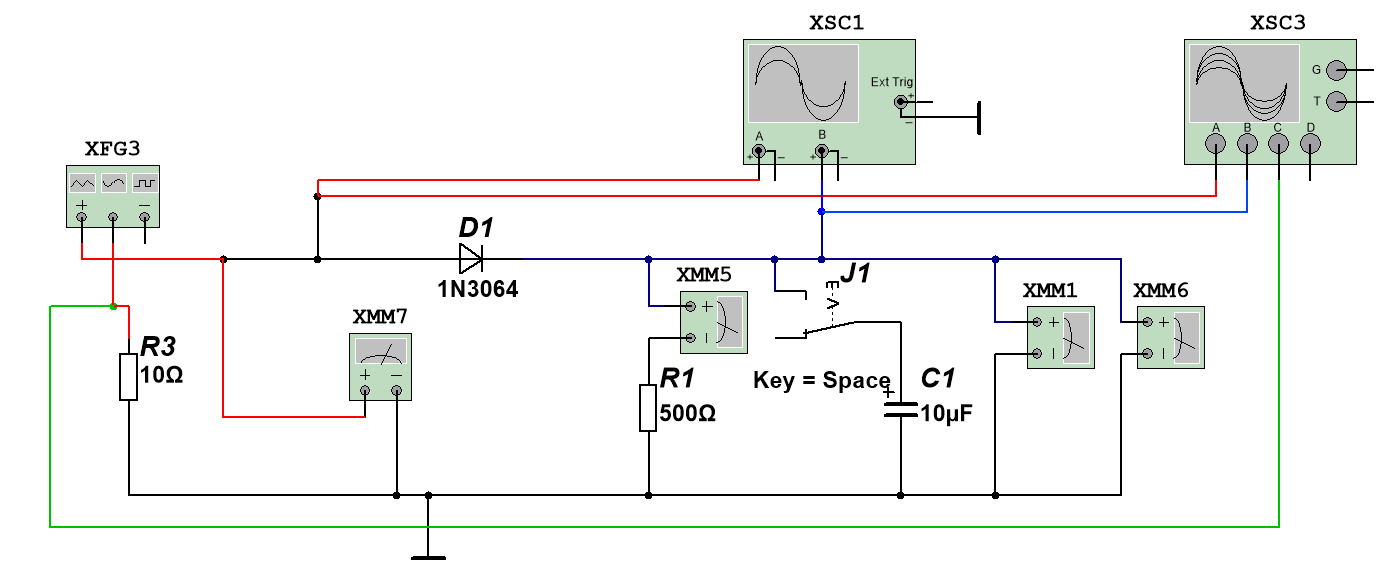
\includegraphics[width=\textwidth]{Scheme.png}
\caption{Схема однополупериодного выпрямителя}
\label{fig:single_half_wave_rectifier}
\end{figure}

\section{Работа однополупериодного выпрямителя на активную нагрузку}

Установлено $E_{\text{г}} = 5$ В, что показано на рисунке \ref{fig:XFG3}. На рисунке 
\ref{fig:XSC3} представлена картина осциллографа XSC3 при работе однополупериодного 
выпрямителя на активную нагрузку в нижнем положении ключа $J_1$.

\begin{figure}[H]
\centering
\begin{subfigure}{0.35\textwidth}
\centering
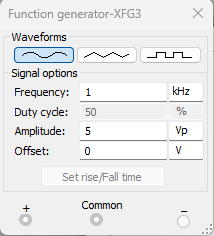
\includegraphics[width=\textwidth]{XFG3.png}
\caption{Генератор XFG3}
\label{fig:XFG3}
\end{subfigure}\hfill
\begin{subfigure}{0.6\textwidth}
\centering
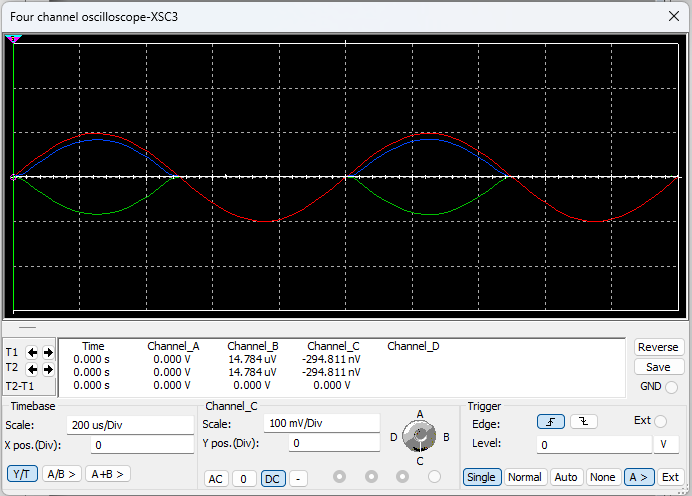
\includegraphics[width=\textwidth]{XSC3.png}
\caption{Картина осциллографа XSC3 при работе однополупериодного выпрямителя на 
активную нагрузку в нижнем положении ключа $J_1$}
\label{fig:XSC3}
\end{subfigure}
\end{figure}

\section{Подключение ёмкостного фильтра}

Нагрузочная характеристика выпрямителя: 
$$U_O=f(I_O)$$

\begin{table}[H]
\centering
\begin{tabularx}{\textwidth}{|>{\centering\arraybackslash}X|>{\centering\arraybackslash}X|>{\centering\arraybackslash}X|>{\centering\arraybackslash}X|>{\centering\arraybackslash}X|>{\centering\arraybackslash}X|>{\centering\arraybackslash}X|}
\hline
$R_{\text{н}}$ & $400$  & $500$ & $600$ & $700$ & $800$ & Ом \\
\hline
$U_O$ & $3.351$ & $3.473$ & $3.562$ & $3.631$ & $3.688$ & В \\
\hline
$I_O$ & $8.378$ & $6.945$ & $5.936$ & $5.187$ & $4.610$ & мА \\
\hline
\end{tabularx}
\end{table}

На рисунке \ref{fig:load_characteristic} представлен график нагрузочной характеристики 
выпрямителя, построенный по данным из таблицы выше. На рисунке \ref{fig:XSC3_2} 
представлена картина осциллографа XSC3 при работе однополупериодного выпрямителя 
на активную нагрузку в верхнем положении ключа $J_1$.


\begin{figure}[H]
\centering
\begin{tikzpicture}
\begin{axis}[
	width=\textwidth,
	height=0.6\textwidth,
	xlabel={$I_O$, мА},
	ylabel={$U_O$, В},
	grid,
	every axis legend/.append style={at={(0.98,0.98)}, anchor=north east}
]
\addplot[
	color=blue,
	mark=*,
	line width=2pt,
	mark size=1pt
] coordinates {
	(8.378, 3.351)
	(6.945, 3.473)
	(5.936, 3.562)
	(5.187, 3.631)
	(4.610, 3.688)
};
\addlegendentry{Нагрузочная характеристика}
\end{axis}
\end{tikzpicture}
\caption{График нагрузочной характеристики выпрямителя}
\label{fig:load_characteristic}
\end{figure}

\begin{figure}[H]
\centering
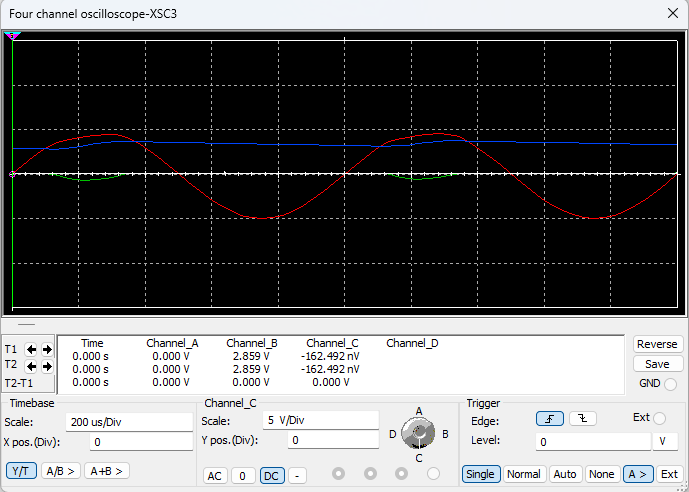
\includegraphics[width=\textwidth]{XSC3_2.png}
\caption{Картина осциллографа XSC3 при работе однополупериодного выпрямителя на 
активную нагрузку в верхнем положении ключа $J_1$}
\label{fig:XSC3_2}
\end{figure}

\section{Определение внутреннего сопротивления выпрямителя}

Внутреннее сопротивление выпрямителя $r_{\text{в}}$ определим по формуле:
$$r_{\text{в}} = \frac{\Delta U_O}{\Delta I_O}$$
где $\Delta U_O$ и $\Delta I_O$ - изменения напряжения и тока на выходе выпрямителя 
при изменении нагрузки. Возьмём точки $R_{\text{н}} = 500$ 
Ом и $R_{\text{н}} = 600$ Ом из таблицы выше.
$$\Delta U_O = 3.562 - 3.473 = 0.089 \text{ В}$$
$$\Delta I_O = 6.945 - 5.936 = 1.009 \text{ мА}$$
Тогда внутреннее сопротивление выпрямителя:

$$r_{\text{в}} = \frac{0.089}{1.009\cdot 10^{-3}} \approx 88.2 \text{ Ом}$$

\section{Определение коэффициента пульсации}

Коэффициент пульсации $P_{\text{пул}}$ определим по формуле:
$$P_{\text{пул}} = \frac{U_{\text{п}}}{U_O}\times 100\%$$
где $U_{\text{п}}$ - амплитуда пульсаций, $U_O$ - среднее значение напряжения на нагрузке.

\begin{table}[H]
\centering
\begin{tabularx}{\textwidth}{|>{\centering\arraybackslash}X|>{\centering\arraybackslash}X|>{\centering\arraybackslash}X|>{\centering\arraybackslash}X|>{\centering\arraybackslash}X|>{\centering\arraybackslash}X|>{\centering\arraybackslash}X|}
\hline
$C_{\text{ф}}, \mu\text{F}$ & $10$ & $20$ & $50$ & $100$ & $150$ & $500$ \\
\hline
$U_{\text{пул}}, \text{мВ}$ & $166.967$ & $84.211$ & $33.834$ & $16.957$ & $11.335$ & $5.456$ \\
\hline
$U_O, \text{В}$ & $3.473$ & $3.500$ & $3.507$ & $3.508$ & $3.508$ & $3.508$ \\
\hline
$P_{\text{пул}}, \%$ & $4.806$ & $2.406$ & $0.964$ & $0.483$ & $0.323$ & $0.155$ \\
\hline
\end{tabularx}
\end{table}

\enlargethispage*{\baselineskip}

На рисунке \ref{fig:pulse_coefficient} представлен график зависимости коэффициента 
пульсации от ёмкости фильтра, построенный по данным из таблицы выше.

\begin{figure}[H]
\centering
\begin{tikzpicture}
\begin{axis}[
	width=\textwidth,
	height=0.6\textwidth,
	xlabel={$C_{\text{ф}}$, мкФ},
	ylabel={$P_{\text{пул}}$, \%},
	grid,
	every axis legend/.append style={at={(0.98,0.98)}, anchor=north east}
]
\addplot[
	color=red,
	mark=*,
	line width=2pt,
	mark size=1pt
] coordinates {
	(10, 4.806)
	(20, 2.406)
	(50, 0.964)
	(100, 0.483)
	(150, 0.323)
	(500, 0.155)
};
\addlegendentry{Коэффициент пульсации}
\end{axis}
\end{tikzpicture}
\caption{График зависимости коэффициента пульсации от ёмкости фильтра}
\label{fig:pulse_coefficient}
\end{figure}

\pagebreak

Зависимость амплитуды пульсаций от частоты генератора:

$$U_{\text{пул}} = f(\nu)$$

\begin{table}[H]
\centering
\begin{tabularx}{\textwidth}{|>{\centering\arraybackslash}X|>{\centering\arraybackslash}X|>{\centering\arraybackslash}X|>{\centering\arraybackslash}X|>{\centering\arraybackslash}X|>{\centering\arraybackslash}X|>{\centering\arraybackslash}X|>{\centering\arraybackslash}X|}
\hline
$\nu$, гЦ & $400$ & $500$ & $600$ & $700$ & $800$ & $900$ & $1000$ \\
\hline
$U_{\text{пул}}$, мВ & $402.880$ & $329.037$ & $277.042$ & $238.670$ & $209.195$ & $185.847$ & $166.964$ \\
\hline
\end{tabularx}
\end{table}

На рисунке \ref{fig:ripple_frequency} представлен график зависимости амплитуды 
пульсаций от частоты, построенный по данным из таблицы выше.

\begin{figure}[H]
\centering
\begin{tikzpicture}
\begin{axis}[
	width=\textwidth,
	height=0.6\textwidth,
	xlabel={$\nu$, гЦ},
	ylabel={$U_{\text{пул}}$, мВ},
	grid,
	every axis legend/.append style={at={(0.98,0.98)}, anchor=north east}
]
\addplot[
	color=green,
	mark=*,
	line width=2pt,
	mark size=1pt
] coordinates {
	(400, 402.880)
	(500, 329.037)
	(600, 277.042)
	(700, 238.670)
	(800, 209.195)
	(900, 185.847)
	(1000, 166.964)
};
\addlegendentry{Амплитуда пульсаций}
\end{axis}
\end{tikzpicture}
\caption{График зависимости амплитуды пульсаций от частоты}
\label{fig:ripple_frequency}
\end{figure}

В первые мгновения после включения наблюдается большая пульсация и малое напряжение на 
нагрузке, что связано с высокой ёмкостью конденсатора фильтра. Через фиксированое время 
пульсация уменьшается, а напряжение на нагрузке увеличивается до своего максимального 
значения, так как конденсатор успевает зарядиться.

\section*{Исследование двухполупериодной схемы выпрямителя}

\begin{figure}[H]
\centering
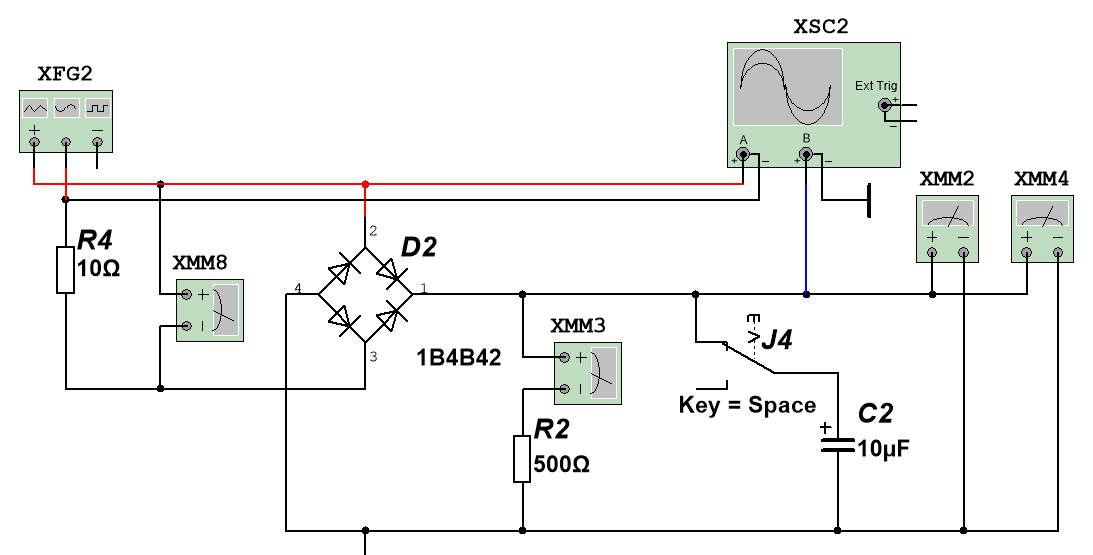
\includegraphics[width=\textwidth]{Scheme2.png}
\caption{Схема двухполупериодного выпрямителя}
\label{fig:double_half_wave_rectifier}
\end{figure}

\section{Работа двухполупериодного выпрямителя на активную нагрузку}

Установлено $E_{\text{г}} = 5$ В, что показано на рисунке \ref{fig:XFG2}. На рисунке 
\ref{fig:XSC2} представлена картина осциллографа XSC2 при работе двухполупериодного 
выпрямителя на активную нагрузку в нижнем положении ключа $J_1$.

\begin{figure}[H]
\centering
\begin{subfigure}{0.35\textwidth}
\centering
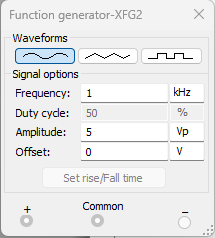
\includegraphics[width=\textwidth]{XFG2.png}
\caption{Генератор XFG2}
\label{fig:XFG2}
\end{subfigure}\hfill
\begin{subfigure}{0.6\textwidth}
\centering
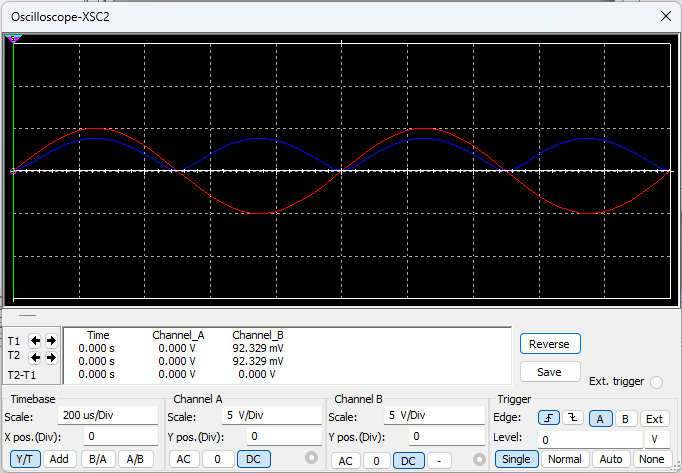
\includegraphics[width=\textwidth]{XSC2.png}
\caption{Картина осциллографа XSC2 при работе двухполупериодного выпрямителя на 
активную нагрузку в нижнем положении ключа $J_1$}
\label{fig:XSC2}
\end{subfigure}
\end{figure}

\section{Подключение ёмкостного фильтра}

Нагрузочная характеристика выпрямителя: 
$$U_O=f(I_O)$$

\begin{table}[H]
\centering
\begin{tabularx}{\textwidth}{|>{\centering\arraybackslash}X|>{\centering\arraybackslash}X|>{\centering\arraybackslash}X|>{\centering\arraybackslash}X|>{\centering\arraybackslash}X|>{\centering\arraybackslash}X|>{\centering\arraybackslash}X|}
\hline
$R_{\text{н}}$ & $400$  & $500$ & $600$ & $700$ & $800$ & Ом \\
\hline
$U_O$ & $3.216$ & $3.305$ & $3.373$ & $3.427$ & $3.473$ & В \\
\hline
$I_O$ & $8.040$ & $6.609$ & $5.621$ & $4.897$ & $4.341$ & мА \\
\hline
\end{tabularx}
\end{table}

На рисунке \ref{fig:load_characteristic_2} представлен график нагрузочной характеристики 
выпрямителя, построенный по данным из таблицы выше. На рисунке \ref{fig:XSC2_2} 
представлена картина осциллографа XSC2 при работе двухполупериодного выпрямителя 
на активную нагрузку в верхнем положении ключа $J_1$.

\begin{figure}[H]
\centering
\begin{tikzpicture}
\begin{axis}[
	width=\textwidth,
	height=0.6\textwidth,
	xlabel={$I_O$, мА},
	ylabel={$U_O$, В},
	grid,
	every axis legend/.append style={at={(0.98,0.98)}, anchor=north east}
]
\addplot[
	color=blue,
	mark=*,
	line width=2pt,
	mark size=1pt
] coordinates {
	(8.040, 3.216)
	(6.609, 3.305)
	(5.621, 3.373)
	(4.897, 3.427)
	(4.341, 3.473)
};
\addlegendentry{Нагрузочная характеристика}
\end{axis}
\end{tikzpicture}
\caption{График нагрузочной характеристики выпрямителя}
\label{fig:load_characteristic_2}
\end{figure}

\begin{figure}[H]
\centering
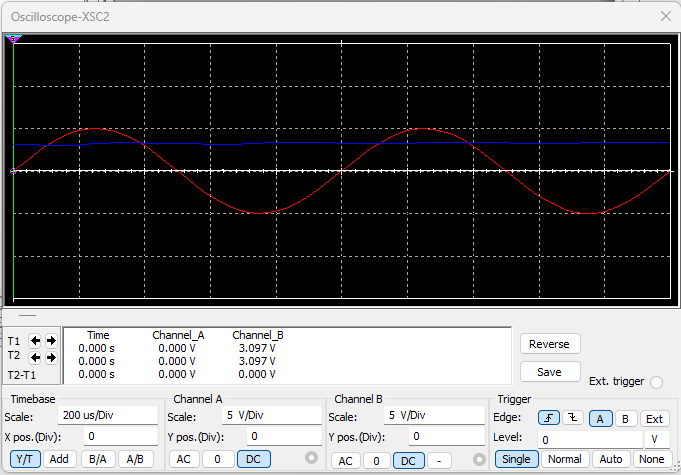
\includegraphics[width=\textwidth]{XSC2_2.png}
\caption{Картина осциллографа XSC2 при работе двухполупериодного выпрямителя на 
активную нагрузку в верхнем положении ключа $J_1$}
\label{fig:XSC2_2}
\end{figure}

\section{Определение внутреннего сопротивления двухполупериодного выпрямителя}

Внутреннее сопротивление выпрямителя $r_{\text{в}}$ определим по формуле:
$$r_{\text{в}} = \frac{\Delta U_O}{\Delta I_O}$$
где $\Delta U_O$ и $\Delta I_O$ - изменения напряжения и тока на выходе выпрямителя 
при изменении нагрузки. Возьмём точки $R_{\text{н}} = 500$ Ом и $R_{\text{н}} = 600$ Ом из таблицы выше.
$$\Delta U_O = 3.373 - 3.305 = 0.068 \text{ В}$$
$$\Delta I_O = 6.609 - 5.621 = 0.988 \text{ мА}$$
Тогда внутреннее сопротивление выпрямителя:
$$r_{\text{в}} = \frac{0.068}{0.988\cdot 10^{-3}} \approx 68.8 \text{ Ом}$$

\section{Определение коэффициента пульсации двухполупериодного выпрямителя}

Коэффициент пульсации $P_{\text{пул}}$ определим по формуле:
$$P_{\text{пул}} = \frac{U_{\text{п}}}{U_O}\times 100\%$$
где $U_{\text{п}}$ - амплитуда пульсаций, $U_O$ - среднее значение напряжения на нагрузке.

\begin{table}[H]
\centering
\begin{tabularx}{\textwidth}{|>{\centering\arraybackslash}X|>{\centering\arraybackslash}X|>{\centering\arraybackslash}X|>{\centering\arraybackslash}X|>{\centering\arraybackslash}X|>{\centering\arraybackslash}X|>{\centering\arraybackslash}X|}
\hline
$C_{\text{ф}}, \mu\text{F}$ & $10$ & $20$ & $50$ & $100$ & $150$ & $500$ \\
\hline
$U_{\text{пул}}, \text{мВ}$ & $65.389$ & $32.803$ & $13.140$ & $6.572$ & $4.382$ & $1.315$ \\
\hline
$U_O, \text{В}$ & $3.305$ & $3.310$ & $3.312$ & $3.312$ & $3.312$ & $3.312$ \\
\hline
$P_{\text{пул}}, \%$ & $2.0$ & $1.0$ & $0.4$ & $0.2$ & $0.1$ & $0.04$ \\
\hline
\end{tabularx}
\end{table}

На рисунке \ref{fig:pulse_coefficient_2} представлен график зависимости коэффициента 
пульсации от ёмкости фильтра, построенный по данным из таблицы выше.

\begin{figure}[H]
\centering
\begin{tikzpicture}
\begin{axis}[
	width=\textwidth,
	height=0.6\textwidth,
	xlabel={$C_{\text{ф}}$, мкФ},
	ylabel={$P_{\text{пул}}$, \%},
	grid,
	every axis legend/.append style={at={(0.98,0.98)}, anchor=north east}
]
\addplot[
	color=red,
	mark=*,
	line width=2pt,
	mark size=1pt
] coordinates {
	(10, 2.0)
	(20, 1.0)
	(50, 0.4)
	(100, 0.2)
	(150, 0.1)
	(500, 0.04)
};
\addlegendentry{Коэффициент пульсации}
\end{axis}
\end{tikzpicture}
\caption{График зависимости коэффициента пульсации от ёмкости фильтра для двухполупериодного выпрямителя}
\label{fig:pulse_coefficient_2}
\end{figure}

Зависимость амплитуды пульсаций от частоты генератора:

$$U_{\text{пул}} = f(\nu)$$

\begin{table}[H]
\centering
\begin{tabularx}{\textwidth}{|>{\centering\arraybackslash}X|>{\centering\arraybackslash}X|>{\centering\arraybackslash}X|>{\centering\arraybackslash}X|>{\centering\arraybackslash}X|>{\centering\arraybackslash}X|>{\centering\arraybackslash}X|>{\centering\arraybackslash}X|}
\hline
$\nu$, гЦ & $400$ & $500$ & $600$ & $700$ & $800$ & $900$ & $1000$ \\
\hline
$U_{\text{пул}}$, мВ & $168.606$ & $135.096$ & $112.269$ & $95.739$ & $83.209$ & $73.339$ & $65.386$ \\
\hline
\end{tabularx}
\end{table}

На рисунке \ref{fig:ripple_frequency_2} представлен график зависимости амплитуды 
пульсаций от частоты, построенный по данным из таблицы выше.

\begin{figure}[H]
\centering
\begin{tikzpicture}
\begin{axis}[
	width=\textwidth,
	height=0.6\textwidth,
	xlabel={$\nu$, гЦ},
	ylabel={$U_{\text{пул}}$, мВ},
	grid,
	every axis legend/.append style={at={(0.98,0.98)}, anchor=north east}
]
\addplot[
	color=green,
	mark=*,
	line width=2pt,
	mark size=1pt
] coordinates {
	(400, 168.606)
	(500, 135.096)
	(600, 112.269)
	(700, 95.739)
	(800, 83.209)
	(900, 73.339)
	(1000, 65.386)
};
\addlegendentry{Амплитуда пульсаций}
\end{axis}
\end{tikzpicture}
\caption{График зависимости амплитуды пульсаций от частоты для двухполупериодного выпрямителя}
\label{fig:ripple_frequency_2}
\end{figure}

\section*{Вывод}
В лабороторной работе были всестороне исследованы конкретные схемы однополупериодного 
и двухполупериодного выпрямителей. Были построены их нагрузочные характеристики, 
определены внутренние сопротивления, а также исследованы зависимости коэффициента 
пульсации от ёмкости фильтра и амплитуды пульсаций от частоты генератора. Полученные 
результаты позволяют сделать вывод о том, что двухполупериодный выпрямитель имеет 
более низкое внутреннее сопротивление и меньший коэффициент пульсации по сравнению 
с однополупериодным выпрямителем, что делает его более эффективным для использования 
в источниках питания. Тем не менее внутренее сопротивление отличается не так 
значительно в сравнении с количеством необходимых дополнительных диодов, а абсолютное 
напряжение пульсаций при сравнимых ёмкостях держится преимущественно на одном 
порядке, так что приминение однополупериодного выпрямителя может быть оправдано 
в случае, если требования к качеству выпрямленного напряжения не высоки.

\end{document}